\documentclass[UTF8]{ctexart}
\usepackage{graphicx} % Required for inserting images
\usepackage{amsmath,amssymb,amsthm}
\usepackage{physics}
\usepackage{graphicx,float}
\graphicspath{{images/}}
\usepackage[none]{hyphenat}
\usepackage{blindtext}
\usepackage{parskip}
\usepackage[letterpaper,top=3cm, left= 3cm,bottom=3cm]{geometry}
\usepackage{subcaption}
\numberwithin{equation}{section}

\begin{document}
\section{高年组简答题:疲倦的光子}
在大爆炸模型提出的早期,有人为了反对大爆炸模型同时解释哈勃定律,提出了“疲倦的光子”假说。该假说认为宇宙是静态的,而光子会随着自己在宇宙中穿梭而失去能量。单位距离内损失的能量由下式表达:
\[
\frac{dE}{dr}=-kE
\]
其中$k$为一常数,$E$为光子的能量。

请证明当$z<<1$,上述假说会给出一个线性的红移-距离关系(即哈勃定律),并求出满足这个条件的$k$。

\subsection{参考答案}
解微分方程,有:
\begin{align*}
    \frac{dE}{dr}&=-kE\\
    \frac{dE}{E}&=-k dr\\
    \int_{E_0}^{E} \frac{dE}{E}&= -k \int_{0}^{r} dr\\
    \ln \frac{E}{E_0} &= -kr\\
    E(r) &= E_0 e^{-kr}
\end{align*}
其中$E_0$为光子初始的能量,$r$是光子走过的距离。

红移和能量也有关系:
\begin{align*}
    z = \frac{\lambda - \lambda_0}{\lambda_0} &= \frac{\frac{hc}{E}-\frac{hc}{E_0}}{\frac{hc}{E_0}}\\
    &= \frac{\frac{1}{E}-\frac{1}{E_0}}{\frac{1}{E_0}}\\
    &= E_0\cdot\frac{E_0-E}{EE_0}\\
    &= \frac{E_0 - E}{E}
\end{align*}
带入能量的表达式,有:
\begin{align*}
    z &= \frac{E_0 - E_0 e^{-kr}}{E_0 e^{-kr}}\\
    &= e^{kr}\left(1-e^{-kr}\right)\\
    &= e^{kr} - 1\\
\end{align*}
当$z<<1$,即$kr<<1$时,有
\begin{align*}
    z \approx kr
\end{align*}
同时带入多普勒效应($v = cz$)
\begin{align*}
    cz &= H_0 r\\
    c kr & = H_0 r\\
    k &= \frac{H_0}{c} = 2.267\cdot 10^{-4} \text{Mpc}^{-1}
\end{align*}

\newpage
\section{普通单选题:第四宇宙速度}
定义第四宇宙速度为从地球发射的卫星逃逸银河系的速度,请求出第四宇宙速度的数值,假设太阳位于银河系的边缘,取银河系质量为$M_{Gal} = 1\cross 10^{12}M_{Sun}$,半径为$R_{Gal} = 33$ kpc

A. 493.927 km/s 

B. 510.628 km/s 

C. 150.483 km/s 

D. 149.559 km/s

\subsection{参考答案}
为了求出第四宇宙速度,先求出第三宇宙速度,地球轨道处逃逸太阳的速度为
\[
v = \sqrt{\frac{2GM_{s}}{R}} = 42.127 \text{ km/s}
\]
考虑到卫星在逃逸的过程中,卫星会获得地球绕转太阳的轨道速度,故在脱离地球引力后,逃离太阳引力所需的速度为
\[
v'_{esc} = \sqrt{\frac{2GM_s}{R}} - \sqrt{\frac{GM_s}{R}} = (\sqrt{2}-1)\sqrt{\frac{GM_s}{R}} = 12.339 \text{ km/s}
\] 
设此时探测器的动能为$E_f$,为了逃离地球,探测器需要达到第二宇宙速度,记探测器逃离地球所需的动能为$E_2$,那么探测器从地球出发,逃离太阳需要的总动能为
\[
E_3 = E_f+E_2
\]
三者的速度则有如下关系
\[
v_3^2 = v'^2_{esc} + v_2^2
\]
其中$v_3$为第三宇宙速度,$v_2$为第二宇宙速度,$v_2 = 11.187 \text{ km/s}$,因此第三宇宙速度为
\[
v_3 = \sqrt{v'^2_{esc} + v_2^2} = 16.655 \text{ km/s}
\]

同理我们可以求出第四宇宙速度,考虑到太阳绕转银河系带来的速度后,银河系边缘的逃逸速度为
\[
v_{esc} = \left(\sqrt{2}-1\right)\sqrt{\frac{GM_{gal}}{R_{gal}}} = 149.559 \text{ km/s}
\]
因此第四宇宙速度为
\[
v_4 = \sqrt{v^2_{esc} + v_3^2} = 150.483 \text{ km/s}
\]
答案为C。

\newpage
\section{低年组单选题:太阳还是黑洞}
如果太阳突然被一个质量相同的黑洞替代,地球的轨道会如何的变化?

A. 什么都不会发生

B. 地球会立刻飞出太阳系

C. 地球会被立刻吸入黑洞

D. 地球的轨道会变成一个离心率更大的椭圆

\subsection{参考答案}
牛顿万有引力定律给出
\[
F = \frac{GMm}{r^2}
\]
其中$M$为中央天体质量,题中说明该质量不变,因此地球受黑洞的引力和受太阳的引力相同,故地球的轨道不会变化。

答案是A。

\newpage
\section{高年组单选:核聚变}
已知恒星的能源来自于核聚变,假设氢原子的动能全部由热运动提供,估算经典条件下发生核聚变的最低温度,假设两个氢原子发生聚变时最近距离为$r = 10^{-15}$ m。

A. $10^8$ K 

B. $10^9$ K 

C. $10^{10}$ K 

D. $10^{11}$ K 

\subsection{参考答案}
气体热运动的平均动能为
\[
K = \frac{3}{2}kT
\]
聚变过程中,氢原子需要克服库伦力势能从而发生聚变,由于库伦力和引力均为平方反比力,其势能形式应该相同。
\[
U = -\frac{1}{4\pi \varepsilon_0} \frac{Q_1 Q_2}{r}
\]
其中$Q$为氢原子的电荷,$Q=e$为基本电荷,如果聚变要发生,动能必须大于势能,否者两原子无法接近彼此,因此边界条件为
\[
\frac{3}{2}kT_{min} -\frac{1}{4\pi\varepsilon_0} \frac{e^2}{r} = 0
\]
解出$T_{min}$, 有
\[
T_{min} = \frac{1}{6\pi \varepsilon_0} \frac{e^2}{kr} \approx 10^{10} \text{ K}
\]
答案是C。

可以发现经典条件下聚变所发生的最低温度远大于太阳核心温度,经典理论在此处失效了。量子隧穿效应可以解释为何太阳核心会发生核聚变,在量子隧穿效应中,一个原子有可能穿过库伦势能构造的势能壁垒,故所需的动能相比经典理论中会大大降低。

\newpage
\section{高年组单选:距离}

通过哈勃定律和多普勒效应,估算$z = 1$处的距离

A. 4282 Mpc

B. 2569 Mpc

C. 7138 Mpc

D. 退行速度为光速,没有对应的物理背景,该问题无意义

\subsection{参考答案}
首先该问题肯定是有意义的,宇宙星体的退行速度是可以超过光速的,因为超光速运动的是膨胀的宇宙,而不是星体,这个假设不违反相对论的基本假设,即物体运动速度不能超过光速。

求这个问题需要引入相对论修正后的红移与速度的关系:
\[
1+z = \sqrt{\frac{c+v}{c-v}}
\]
解$v$,有
\[
v = \frac{(1+z)^2-1}{(1+z)^2+1}c
\]
带入$z=1$,有 
\[
v = \frac{2^2-1}{2^2+1}c = \frac{3}{5}c
\]
求出退行速度后,带入哈勃定律
\[
d = \frac{v}{H_0} = \frac{3}{5} \frac{c}{H_0} = 2569 \text{ Mpc}
\]
答案是B

\newpage
\section{普通简答题:太阳核心}
假设太阳保持流体静力平衡,并且太阳核心是理想气体,估算
\begin{enumerate}
    \item 太阳核心的压强
    \item 太阳核心的粒子数密度
    \item 太阳核心的粒子数密度与地球大气粒子数密度的比
\end{enumerate}
太阳核心温度为$T_c=10^7$ K。

提示:流体静力平衡方程为:
\[
\frac{dP}{dr}=-\frac{GM(r)\rho(r)}{r^2}
\]
等式左端本质上这是一个导数(可以理解为斜率),但是在粗略近似(意味着你可以忽略掉某些系数)情况下,取$dP\approx P_c-P_s$为太阳核心压力与表面压力的差,$dr\approx r_c-r_s$为太阳核心半径与表面半径的差,取$M$为恒星的质量,$\rho$为恒星的平均密度

如果你不会,考虑从量纲方面下手,压力与引力常数$G$,恒星质量$M$和恒星半径$R$相关

\newpage
\subsection{参考答案}
\begin{enumerate}
    \item 注意到$P_s=0$且$r_c=0$(恒星的压力由引力提供,恒星表面没有物质,因此没有压力)于是,有
\[
\frac{P_s}{-R}\approx -\frac{GM\rho}{R^2} 
\]
带入密度的定义,有
\[
\frac{P_s}{R} \approx \frac{GM}{R^2} \cdot \frac{M}{4/3\pi R^3}
\]
化简得出
\[
P_c \approx \frac{GM^2}{R^4} =1.135 \cdot 10^{15} \text{ Pa}
\]

这里的系被忽略掉了(导数都被近似成了斜率还留着系数干啥),提示中说了忽略系数,因此系数必须忽略掉,用量纲的角度就会直接得到这个式子。

\item 根据理想气体方程
\[
PV=Nk_B T
\]
数密度定义为$n = \displaystyle\frac{N}{V}$,为单位体积内粒子的数量,可以得出:
\[
n=\frac{P}{k_B T}=8.221\cdot 10^{30}/m^3
\]

\item 假设地球大气为理想气体 地球大气压$P_E=10^5$ Pa,地球大气温度取$T_E=300$ K,根据理想气体方程
\[
n_Ev= \frac{P_E}{k_B T_E }=2.414 \cdot 10^{25}/m^3
\]
两个数密度相比,有:
\[\frac{n}{n_E} =340555\]
\end{enumerate}

\newpage
\section{普通简答题:变轨}
考虑一颗卫星,在一个椭圆轨道上绕地球公转,半长轴$a_1 = 15000$km,偏心率$e_1 = 0.2$(称其为旧轨道)。卫星需要变轨到一个新的椭圆轨道,半长轴为$a_2 = 25000$km,偏心率为$e_2 = 0.4$(称其为新轨道),两轨道共面。

已知第一次变轨位于旧轨道的近日点,第二次变轨位于新轨道的半短轴处,请求出两次变轨需要的速度增量,以及速度增量与速度矢量的夹角

提示:变轨时速度矢量不一定共线

\subsection{参考答案}
假设变轨时,卫星的轨道也为椭圆,我们可以通过这个求出变轨轨道的极坐标方程。

设变轨轨道的极坐标方程为
\[
r = \frac{a(1-e^2)}{1+e\cos \theta}
\]
这个轨道近日点与旧轨道近日点重合,即
\[
\frac{a(1-e^2)}{1+e\cos 0} = a_1(1-e_1) = 12000 \text{ km}
\]
该轨道的另外一点位于新轨道的半短轴处,我们需要先求出来第二次变轨瞬间的卫星的极坐标。

位于椭圆半短轴处的点距离椭圆焦点的距离是椭圆的半长轴,因此$r_2 = a_2 = 25000$km,此时其极角的余弦值为
\[
\cos \theta_2 = \frac{1}{e_2} \frac{a_2(1-e^2_2)}{r_2} - 1= -\frac{2}{5}
\]
因此得出第二个关于变轨轨道的方程
\[
r_2 = \frac{a(1-e^2)}{1+e\cos \theta_2} = 25000 \text{ km}
\]
联立两方程,有
\[
\begin{cases}
    \displaystyle
    \frac{a(1-e^2)}{1+e\cos 0} = a_1(1-e_1) = 12000 \text{ km}\\
    \displaystyle
    r_2 = \frac{a(1-e^2)}{1+e\cos \theta_2} = 25000 \text{ km}\\
\end{cases}
\]
解出
\[
\begin{cases}
    a = 29333 \text{ km}\\
    e = 0.591\\
\end{cases}
\]
\begin{figure}[H]
    \centering
    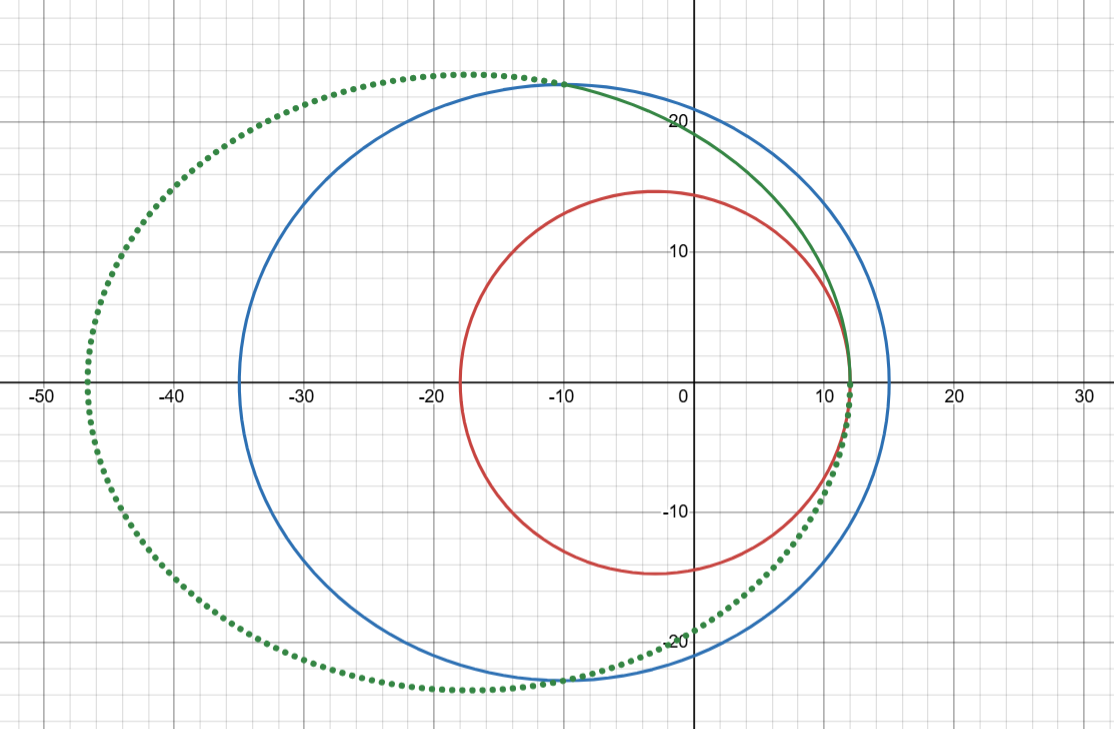
\includegraphics[width = 15cm]{orbitchange.png}
    \caption{变轨示意图}
\end{figure}
上图是变轨示意图,红色的是旧轨道,蓝色的是新轨道,实线绿色的是卫星实际上走过的变轨轨道,虚线绿色是卫星完整的变轨轨道

根据活力公式可以解出第一次变轨所需的速度
\[
v_1 = \sqrt{GM \left(\frac{2}{r_1} - \frac{1}{a_1}\right)} = 6314.02 \text{ m/s}
\]
\[
v_{peri} = \sqrt{GM \left(\frac{2}{r_1} - \frac{1}{a}\right)} = 7270.050 \text{ m/s}
\]
速度增量为
\[
\Delta v_1 = v_{peri} - v_1 = 956.030 \text{ m/s}
\]
此时速度矢量共线,故速度增量与速度矢量的夹角为0

同样可以求出第二次变轨所需的速度,但是需要注意到这次变轨时,速度矢量并不重合
\[
v_2 = \sqrt{GM \left(\frac{2}{r_2} - \frac{1}{a_2}\right)} = 3993.337 \text{ m/s}
\]
\[
v = \sqrt{GM \left(\frac{2}{r_2} - \frac{1}{a}\right)} = 4378.125 \text{ m/s}
\]
现在需要求出来两个速度矢量的夹角,最直观的想法当然是通过求导求出来夹角的大小,但是我们可以用角动量守恒来处理(及开普勒第二定律)
\[
L = m v_{peri}r_1 = m v r_2 \sin \alpha
\]
其中$\alpha$是第二次变轨前速度矢量和位置矢量的夹角,因此可以解出$\alpha$
\[
\alpha = \arcsin (\frac{v_{peri}}{v} \cdot \frac{r_1}{r_2}) = 52.850^\circ
\]
因此速度矢量和位置矢量的夹角为
\[
\beta = \pi - \alpha = 127.15^\circ
\]
两个速度矢量的夹角为
\[
\gamma = \beta - \frac{\pi}{2} = 37.15^\circ
\]
根据余弦定理,变轨所需的速度为
\[
\Delta v_2 = \sqrt{v^2 + v_2^2 - 2vv_2 \cos \gamma} = 2691.522 \text{ m/s}
\]
考虑到卫星在此处需要减速,$\Delta v = -2691.522$ m/s
与$v$的夹角为
\[
\sin i = \frac{v_2}{\Delta v} \sin \gamma
\]
解出$i = 63.637^\circ$
\end{document}